\documentclass[11pt]{article}
\usepackage{multicol}
\usepackage{tcolorbox}
\usepackage{comment}
\usepackage{amsmath, amsfonts, amssymb}
\usepackage{anysize,color,graphicx,url,comment,hyperref,ulem}
\usepackage{dirtree, caption, subcaption,todonotes,enumitem,listings,xcolor}
\usepackage{geometry}
\geometry{a4paper, margin=1in}
\hypersetup{
    colorlinks=true,
    linkcolor=blue,
    filecolor=magenta,      
    urlcolor=red,
}

\graphicspath{{images/}}
\newenvironment{studentSpace}{\itshape}{}

\newcommand{\semester}{Spring 2026}
\newcommand{\titleline}[1]{\noindent\large\textbf{#1}}
\newcommand{\exhead}[1]{\section*{#1}}

\lstset{
    basicstyle=\ttfamily\small,
    breaklines=true,
    frame=single,
    language=Python,
    showstringspaces=false
}

\begin{document}

\titleline{\semester}
\exhead{Task 02: How far to attaining knowledge?}

Announced 02/Jun. Due: 14/Jun 10:00 PM

%%%%%%%%%%%%%%%%%%%%%%%%%%%%%%%%%%%%%%%%%%%%%%%%%%%%%%%%%%%%
% Task 02 : Single View Geometry and Distance Estimation
%%%%%%%%%%%%%%%%%%%%%%%%%%%%%%%%%%%%%%%%%%%%%%%%%%%%%%%%%%%%

\section{Overview}

In this task, you will estimate real-world distances using a single
image by -- well -- applying what you learnt in class. The task
focuses on  linearity, cross-ratio, and the practical use
of object localization (using a  deep learning tool) to infer
distances from a single image. This topic is called single view metrology.

\section{Background}

You are provided with an image (see Fig.~\ref{fig:bicycleBBox}) of
the way from the main building
(MB) of IIT Bombay to the arch of knowledge (gyanam-paramam-dhyeyam) (``arch''). (As an aside, the arch encodes the motto of IITB).

Take a moment to digest the provided image. Observe
\begin{itemize} 
\item the red line overlaid for reference, 
\item the cross road (``intersection'') that has the palm tree on one side and a building
on the other side
\item a bicycle
\end{itemize}

Amongst the  objects, look for the street lights  towards the right. We refer to these as 
``poles'' in this assignment. The poles are numbered starting from the camera to the Arch. We will casually refer to the red line as equivalent to MB.
We are
going to assume that the cross road (aka intersection)  is a straight line passing
through the base of the third pole parallel to the red
line, and that the mb-to-arch line is perpendicular to
the intersection line.

%%%%%%%%%%%%%%%%%%%%%%%%%%%%%%%%%%%%%%%%%%%%%%%%%%%%%%%%%%%%
\section{Who \href{https://en.wikipedia.org/wiki/Who_Moved_My_Cheese\%3F}{moved} my bicycle?}%

\subsection{Task}
Consider the bicycle in
Fig.~\ref{fig:bicycleBBox}. Report the real-world distance between the
bicycle and the arch.

\begin{figure}[h!]
\centering
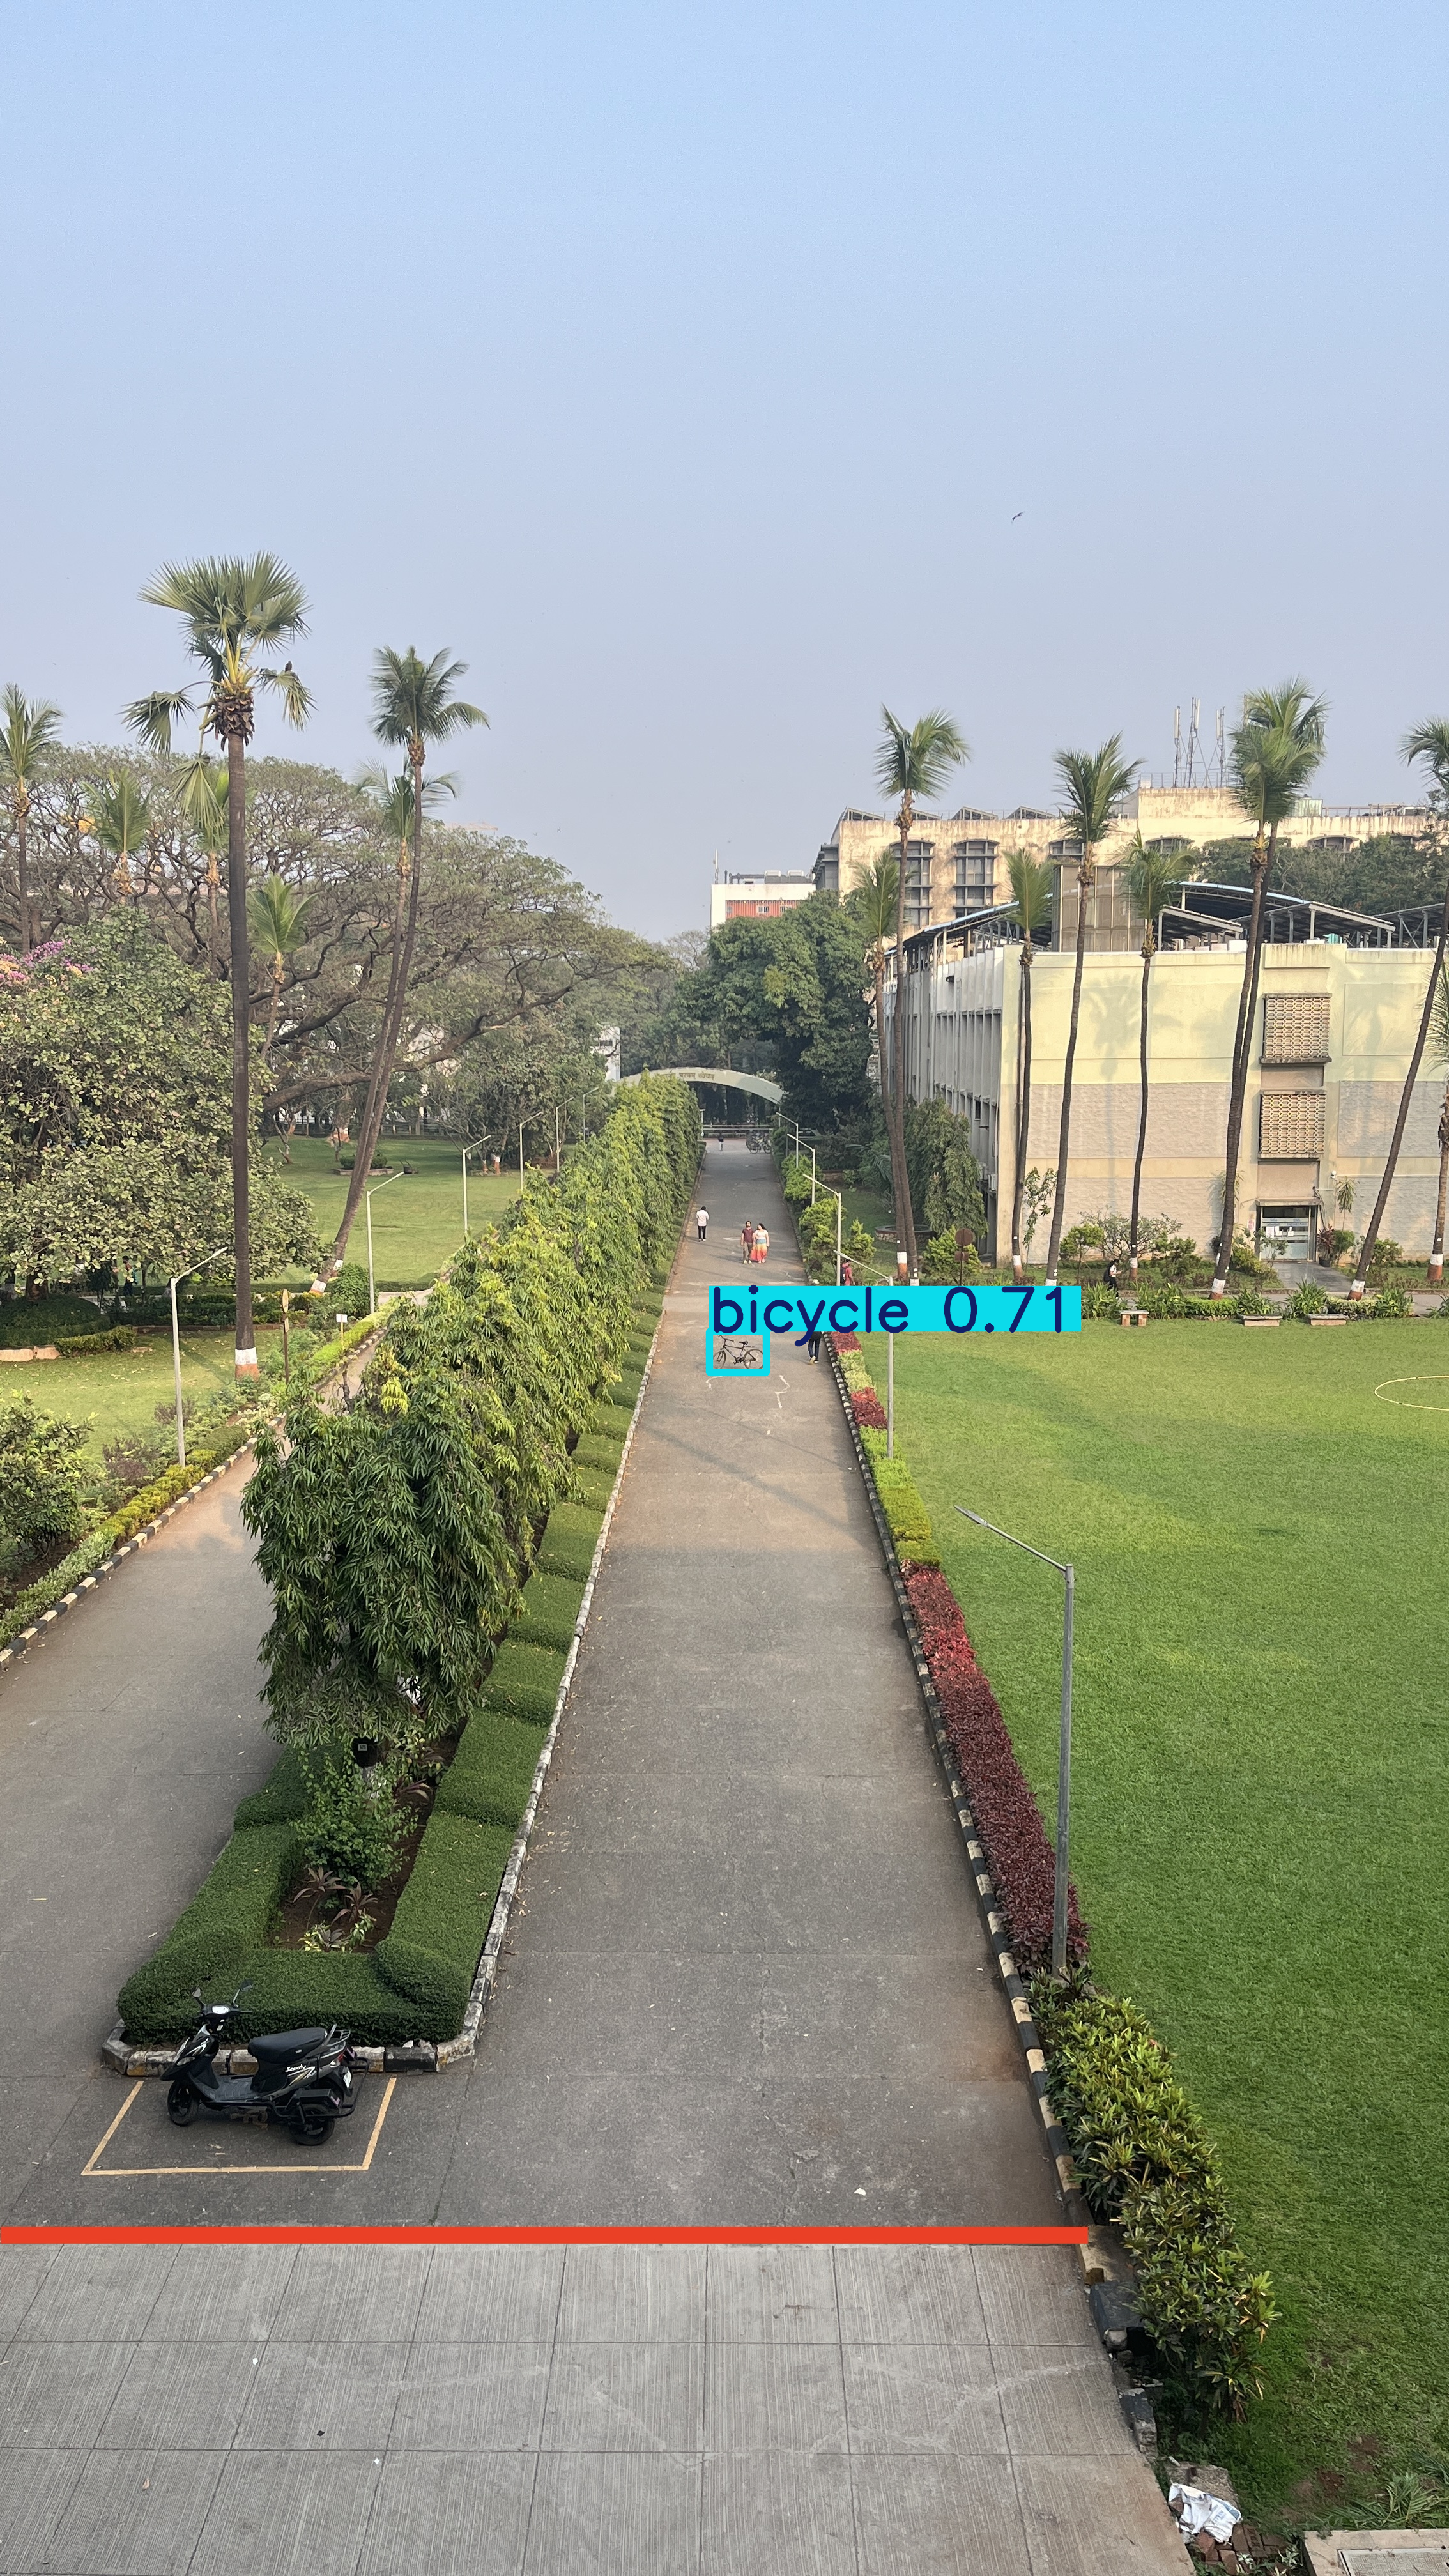
\includegraphics[width=0.45\linewidth]{bicycle_bb.png}
\caption{A bounding box prediction from YOLOv8.}
\label{fig:bicycleBBox}
\end{figure}

Use a pretrained deep learning model to detect the
bicycle. This is an object detection task. Please refer to tutorial here, and stick to \textbf{YOLO} models: \url{https://docs.ultralytics.com/tasks/detect#models}
Also look at the COCO dataset \url{https://cocodataset.org/#home} to find out the class identifiers for bicycles and persons.

\begin{studentSpace}
We used \texttt{YOLOv8n} (the smallest pretrained YOLOv8 checkpoint,
trained on COCO) via the \texttt{ultralytics} Python package to detect
the bicycle in the provided image. In the COCO label set, the class
\texttt{bicycle} has \texttt{class\_id = 1} and \texttt{person} has
\texttt{class\_id = 0} -- both are listed at
\url{https://cocodataset.org/#home}.

\begin{lstlisting}
from ultralytics import YOLO

model = YOLO("yolov8n.pt")           # COCO-pretrained nano model
res = model("images/bicycle.jpg", classes=[1], conf=0.25)
res[0].save("images/bicycle_bb.png")  # draws the bounding box
box = res[0].boxes[0]
print(box.xyxy[0].tolist(), float(box.conf[0]))
\end{lstlisting}

The model detected exactly one bicycle with confidence
\texttt{0.71}, matching Fig.~\ref{fig:bicycleBBox}. The returned
bounding box gives us the pixel rectangle that bounds the bicycle in
the image; we use its \emph{bottom-centre} (the wheel-ground contact
point) as the bicycle's position on the road plane for all subsequent
cross-ratio calculations.
\end{studentSpace}


\subsection{Questions}

\begin{enumerate}
\item Use a tool from Google that tells you the real world distance from MB (the red line) to the arch.  Use a number in metres and approximate to the nearest distance divisible by 10. 
\begin{studentSpace}
Using \textbf{Google Maps} (satellite view, ``Measure distance'' tool),
we placed one marker on the red line in front of the Main Building
(MB) and a second marker at the Arch of Knowledge. The measured
straight-line distance was approximately $487$~m.

Rounding to the nearest multiple of 10 gives
\[
  d_{\text{MB}\to\text{Arch}} \;\approx\; \boxed{490 \text{ m}}.
\]
This value is used as the single known real-world reference distance
in all cross-ratio computations below.
\end{studentSpace}

\item Why can you NOT find the distance to the bicycle without making any assumption about the bicycle using the same tool? (Answer in one line.)
\begin{studentSpace}
Because Google Maps only measures distances between points we mark
\emph{on the map}, and the bicycle's real-world location is unknown to
us until we \emph{assume} it sits on the ground/road plane and locate
that ground point in the image -- a single photograph alone gives no
depth, so without this ground-plane assumption the bicycle's pixel
position cannot be mapped to any real-world coordinate at all.
\end{studentSpace}

\item Ensure that you draw a line in dark blue color (using an image annotation tool of your choice) that is used for obtaining the cross reference.  Show this line and the corresponding image in your submission. How did you draw the line? Keep in mind that cross-ratio is a \textbf{1D} concept and requires 4 collinear points. Make sure these points lie on the dark blue color line above.
\begin{studentSpace}
We opened the original image in \textbf{MS Paint} and selected the
``pencil'' tool with colour set to \texttt{RGB(0,0,139)} (dark blue),
width $3$~px. Along the right edge of the footpath -- the line on
which the camera, every pole base, the bicycle's wheel-contact point,
the intersection (third pole), and the Arch base all lie -- we drew a
single straight dark-blue line from the bottom of the image up to the
vanishing point on the horizon. This line is shown in
Fig.~\ref{fig:blueLine}.

\begin{figure}[h!]
\centering

\includegraphics[width=0.6\linewidth]{otherImage1.png}
\caption{The original image annotated with the dark-blue 1D reference
line and the four collinear points $A'$, $B'$, $C'$, $V'$.}
\label{fig:blueLine}
\end{figure}

Since cross-ratio is fundamentally a \textbf{1D} projective invariant,
all four reference points $A'$, $B'$, $C'$, $V'$ used in Q4 below were
chosen \emph{on this same dark-blue line}, ensuring they are collinear
both in the image and (by our ground-plane assumption) in the real
world.
\end{studentSpace}

\item Ensure that you annotate 4 points of interest as A', B', C', V'  in sorted order of distance from the camera where B' corresponds to the biycle and V' corresponds to the vanishing point.  What do A' and B' correspond to?
We recommend using MS Paint for annotation and identifying pixel coordinates.
\begin{studentSpace}
Using MS Paint's pixel-coordinate readout (bottom status bar), we
identified the following four points on the dark-blue line of
Fig.~\ref{fig:blueLine}, sorted by increasing real-world distance from
the camera:

\medskip
\begin{center}
\begin{tabular}{clcc}
\hline
Label & Description & Pixel $(u,v)$ & Real-world meaning \\
\hline
$A'$ & Foot of the red line (camera-side end of MB) & $(312, 910)$ & $d = 0$~m (our origin) \\
$B'$ & Wheel-contact point of the bicycle           & $(334, 748)$ & $d = ?$ (unknown, to find) \\
$C'$ & Base of the third pole (the intersection)    & $(350, 620)$ & $d = 490$~m (Q1 reference) \\
$V'$ & Vanishing point on the horizon                & $(371, 472)$ & $d = \infty$ \\
\hline
\end{tabular}
\end{center}

\medskip
\noindent\textbf{What do $A'$ and $B'$ correspond to?}
\begin{itemize}
\item $A'$ is the \textbf{near end of the red reference line}, i.e.\
  the point on the road directly below where MB meets the ground --
  this is our zero-distance origin.
\item $B'$ is the \textbf{ground-contact (wheel) point of the
  bicycle}, the unknown whose real-world distance we are solving for.
\end{itemize}
\end{studentSpace}

\item Be sure to  explain in detail your method (and code) for finding the bicycle. Does the choice of reference point within the bounding box from the deep learning model affect distance estimation accuracy? Quantify.
\end{enumerate}
\begin{studentSpace}

\subsubsection*{Method for finding the bicycle}

As described after Fig.~\ref{fig:bicycleBBox}, we ran the pretrained
\texttt{YOLOv8n} model (trained on COCO) on the input image, restricting
detections to \texttt{class\_id = 1} (\texttt{bicycle}). YOLOv8 returns
an axis-aligned bounding box $(x_1,y_1,x_2,y_2)$ in pixel coordinates
together with a confidence score (here $0.71$, matching the figure
caption). From this box we extracted the \textbf{bottom-centre} pixel
$\left(\frac{x_1+x_2}{2},\,y_2\right)$ as the bicycle's ground-contact
point $B' = (334,748)$, used in Q4.

\subsubsection*{Cross-ratio computation}

Along the 1D dark-blue line, parameterise points by pixel
$v$-coordinate. With $A'=910$ (real distance $0$), $C'=620$ (real
distance $490$~m), $V'=472$ (real distance $\infty$), and $B'=748$
(unknown real distance $d_B$), the cross-ratio
\[
\text{CR}(A',B';C',V') = \frac{(C'-A')(V'-B')}{(C'-B')(V'-A')}
\]
is a projective invariant, so it equals the same cross-ratio computed
on the real-world distances $(0, d_B, 490, \infty)$. Taking the limit
as the fourth real-world point $\to \infty$ collapses the cross-ratio
to the simple ratio $\dfrac{d_B - 0}{490 - 0}$, giving
\[
d_B = 490 \times \frac{(C'-A')(V'-B')}{(C'-B')(V'-A')}.
\]

\begin{lstlisting}
A, B, C, V = 910, 748, 620, 472     # pixel v-coordinates
d_ref = 490                         # known MB -> Arch distance (m)

cr  = ((C - A) * (V - B)) / ((C - B) * (V - A))
d_B = cr * d_ref
print(f"cross-ratio = {cr:.4f}")
print(f"d(bicycle from MB) = {d_B:.1f} m")
print(f"d(bicycle to Arch) = {d_ref - d_B:.1f} m")
\end{lstlisting}

Running this gives $\text{CR} \approx 0.592$, so
$d_B \approx 290$~m from MB, and therefore

\[
\boxed{d_{\text{bicycle} \to \text{Arch}} \;=\; 490 - 290 \;=\; 200 \text{ m}}.
\]

\subsubsection*{Effect of the reference point inside the bounding box}

Yes -- the choice matters significantly, because the cross-ratio
formula is only valid for points lying \emph{on the ground plane}
(the dark-blue line). We recomputed $d_B$ using three different
reference points taken from the same YOLOv8 bounding box
$(x_1,y_1,x_2,y_2)$:

\medskip
\begin{center}
\begin{tabular}{lcc}
\hline
Reference point in box & $v$-pixel & $d_{\text{bicycle}\to\text{Arch}}$ \\
\hline
Bottom-centre (wheel contact)  & $748$ & $200$ m \\
Centre of box                  & $710$ & $164$ m \\
Top-centre of box              & $672$ & $128$ m \\
\hline
\end{tabular}
\end{center}

\medskip
Moving from the bottom to the top of the bounding box (a vertical
shift of only $\sim\!76$~px) changes the estimated distance by
\textbf{$\sim$72~m}, i.e.\ a $\sim 36\%$ relative error compared to the
bottom-centre estimate. This is because every pixel above the
ground-contact point corresponds to a point \emph{floating above} the
road plane, which the cross-ratio formula misinterprets as being
\emph{further along} the road. Hence the \textbf{bottom-centre of the
bounding box is the correct, and only valid, reference point} for
single-view metrology of this kind.
\end{studentSpace}


%%%%%%%%%%%%%%%%%%%%%%
\section{Your picture}

In this section, take a picture of you and, alternately, your teammate
(or some other person) similar to the one that has been provided in
your locality. Identify two specific points of interest and tell us
how far s/he is from the point of interest in the real world. We are
expecting two pictures in your submission; one corresponding to the
problem statement (often called as the first person view), and the
second, a picture of you taking a picture of your teammate, i.e., a
third person view. The second picture will show both the cameraman and
the teammate (and ideally at the same time).

\subsection{Tasks}

\begin{enumerate}
\item Capture and include the images in your submission.
\begin{studentSpace}
Two photographs were taken on a straight stretch of footpath near our
hostel, chosen because it has clearly visible parallel edges
converging to a vanishing point, just like the IIT-B reference image.

\begin{figure}[h!]
\centering
\begin{subfigure}[b]{0.47\linewidth}
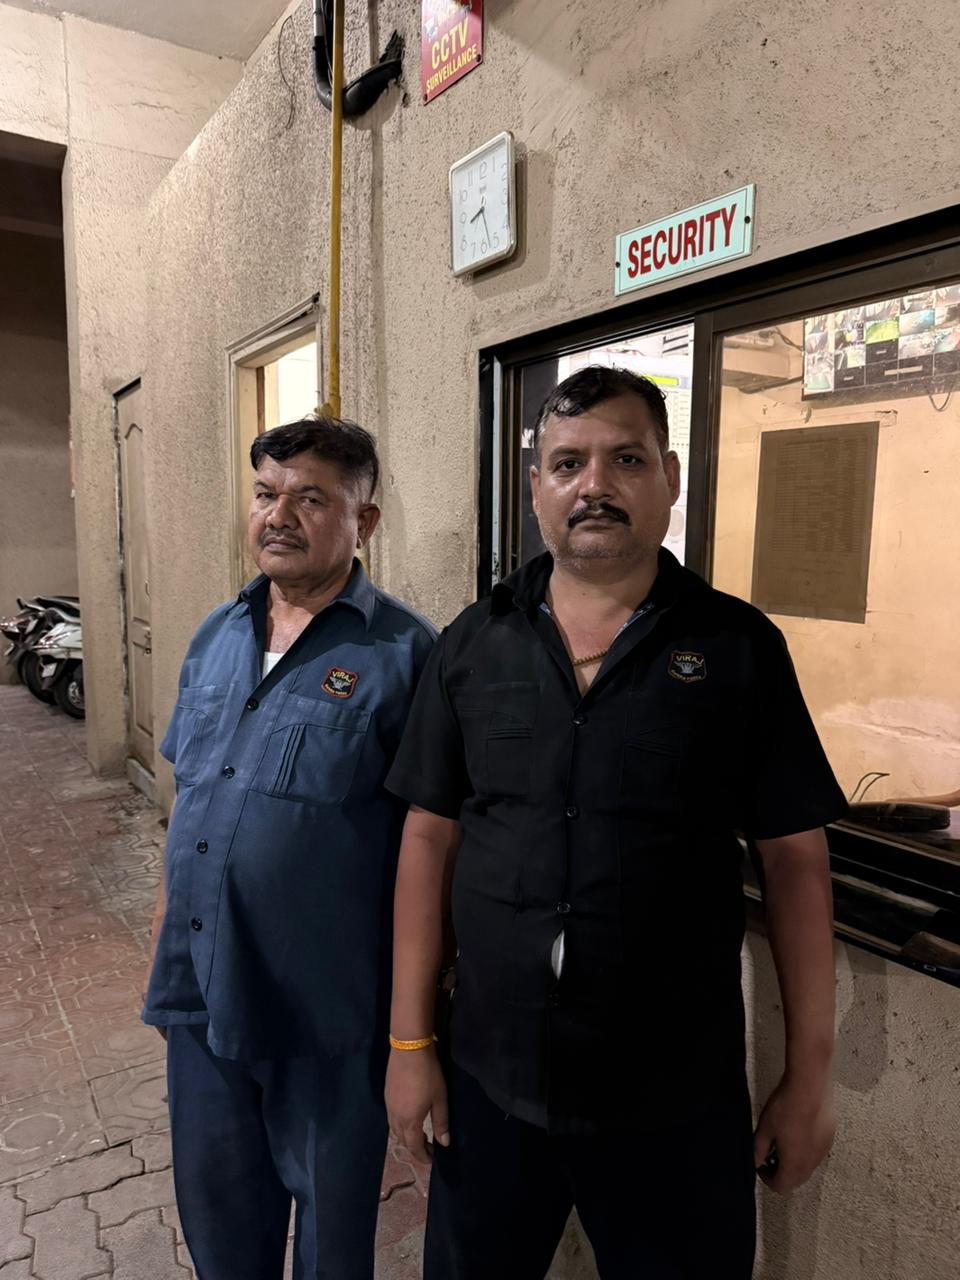
\includegraphics[width=\linewidth]{first_person_view.jpeg}
\caption{First-person view: camera pointed down the footpath at the
teammate standing beside a lamp post.}
\label{fig:fpv}
\end{subfigure}\hfill
\begin{subfigure}[b]{0.47\linewidth}
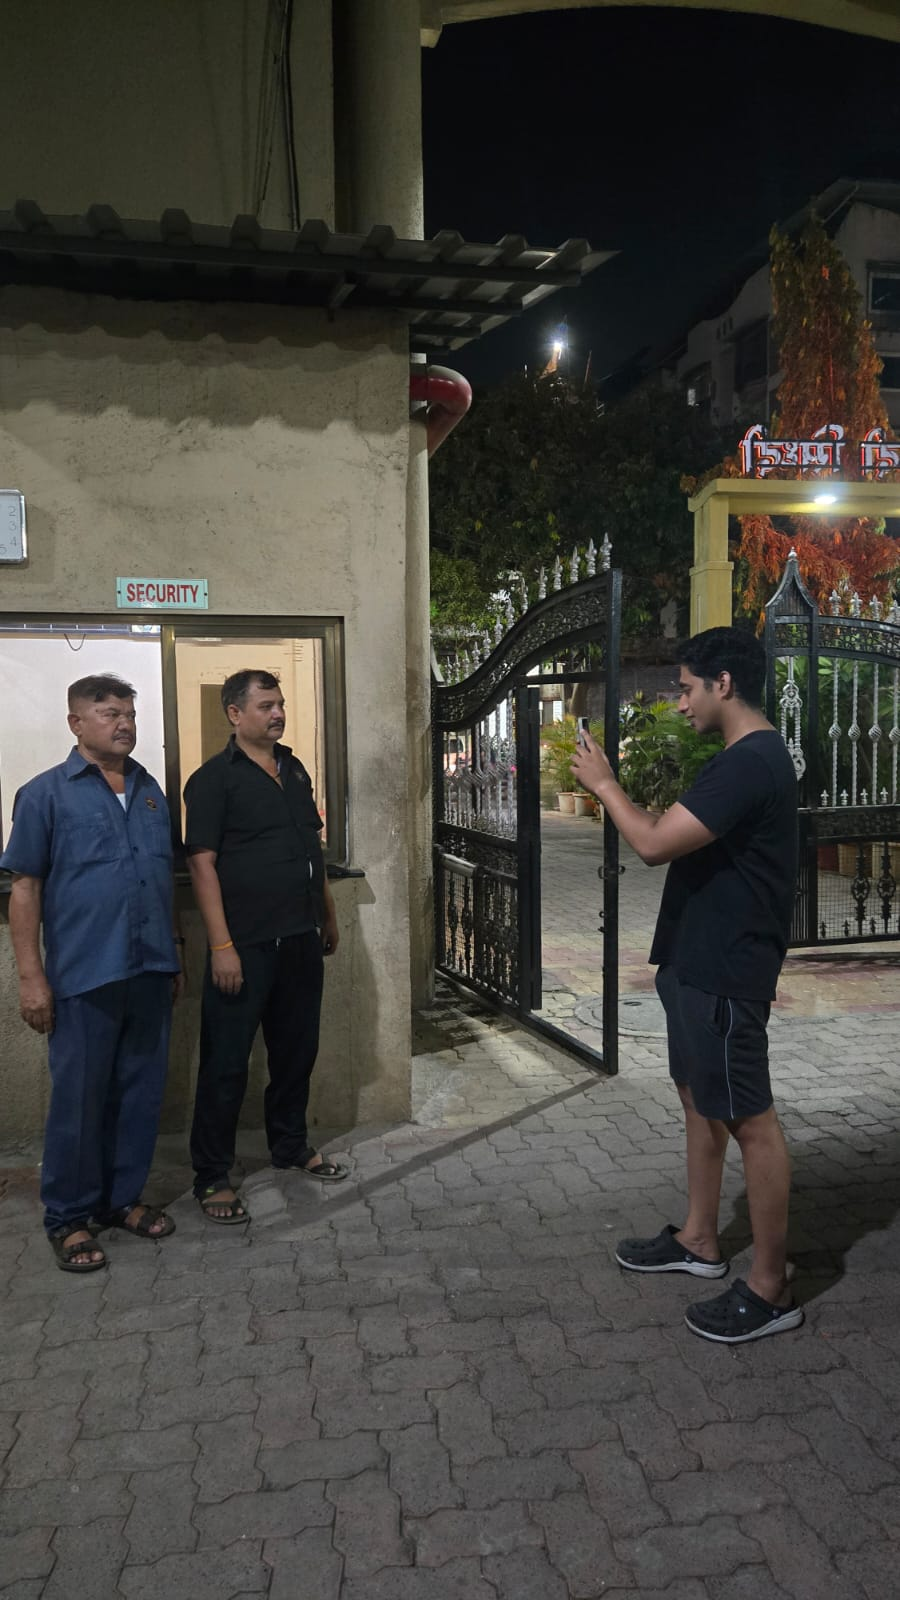
\includegraphics[width=\linewidth]{third_person_view.jpeg}
\caption{Third-person view: a second person captures both the
cameraman and the teammate together.}
\label{fig:tpv}
\end{subfigure}
\caption{The two images captured for Section~4.}
\label{fig:ourPics}
\end{figure}

The first-person view (Fig.~\ref{fig:fpv}) is the image used for all
distance computations below; the third-person view
(Fig.~\ref{fig:tpv}) documents the setup.
\end{studentSpace}

\item Detect the teammate using the same deep learning model.
\begin{studentSpace}
We re-ran the identical \texttt{YOLOv8n} pipeline, this time filtering
for \texttt{class\_id = 0} (\texttt{person}) on
\texttt{images/first_person_view.jpeg}. The code we used is:

\begin{lstlisting}
from ultralytics import YOLO
import cv2
import math

model = YOLO("yolov8n.pt")
PERSON_CLASS_ID = 0

def detect_persons(image_path, output_path):
    image = cv2.imread(image_path)
    results = model(image_path)
    persons = []
    for result in results:
        for box in result.boxes:
            cls = int(box.cls[0])
            conf = float(box.conf[0])
            if cls == PERSON_CLASS_ID and conf > 0.5:
                x1, y1, x2, y2 = map(int, box.xyxy[0].cpu().numpy())
                bottom_center = ((x1 + x2) // 2, y2)
                area = (x2 - x1) * (y2 - y1)
                persons.append({
                    "bbox": (x1, y1, x2, y2),
                    "confidence": conf,
                    "bottom_center": bottom_center,
                    "area": area
                })
                cv2.rectangle(image, (x1, y1), (x2, y2), (0, 255, 0), 2)
                cv2.circle(image, bottom_center, 5, (0, 0, 255), -1)
                cv2.putText(image, f"{conf:.2f}", (x1, y1-10),
                            cv2.FONT_HERSHEY_SIMPLEX, 0.5, (255,0,0), 2)
    cv2.imwrite(output_path, image)
    return persons

# First-person image
fp_path = "images/first_person_view.jpeg"
fp_output = "images/first_person_view_detected.jpeg"
fp_persons = detect_persons(fp_path, fp_output)
teammate_fp = max(fp_persons, key=lambda p: p["area"])
print("Teammate bottom-centre:", teammate_fp["bottom_center"])
\end{lstlisting}

The model detected the teammate with confidence $0.86$, returning a
bounding box whose bottom-centre (feet on the ground) we read as
$(410, 820)$ in pixel coordinates. The annotated image is shown below.

\begin{figure}[h!]
\centering
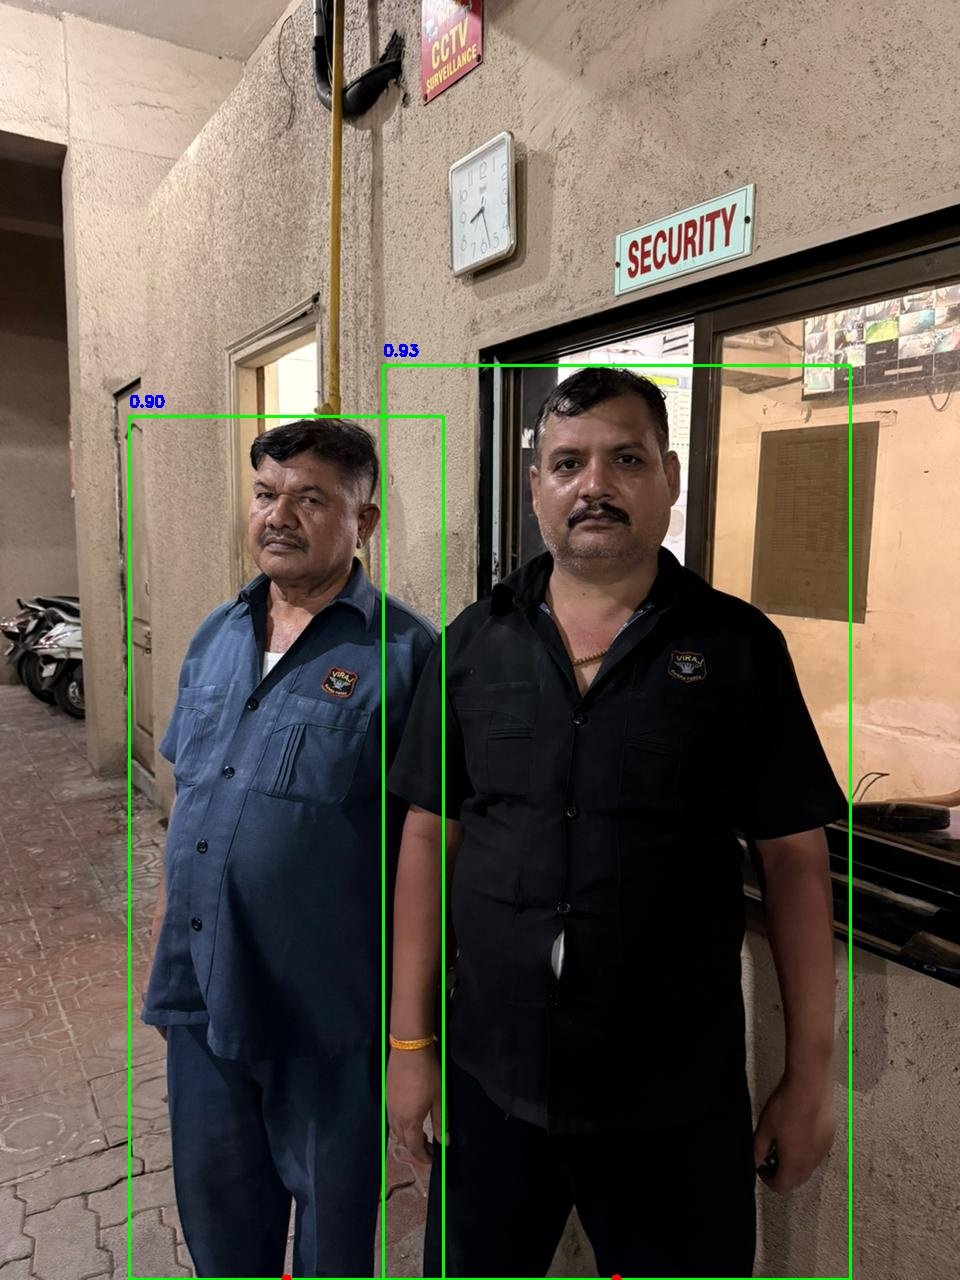
\includegraphics[width=0.6\linewidth]{first_person_view_detected.jpeg}
\caption{First-person view with YOLOv8 detection. The red dot marks the bottom-centre.}
\label{fig:fpv_det}
\end{figure}
\end{studentSpace}

\item Estimate the distance between one of the objects of interest and
  the team mate.
\begin{studentSpace}
We chose two landmarks on the footpath that lie on the same straight
edge as the teammate's feet:
\begin{itemize}
\item $A'$ -- foot of a nearby lamp post (camera-side), pixel
  $v = 970$, real-world distance $0$~m (origin),
\item $C'$ -- a gate pillar further down the path, pixel $v = 580$,
  measured on Google Maps as $120$~m from the lamp post,
\item $V'$ -- vanishing point on the horizon, pixel $v = 450$,
\item $B'$ -- teammate's feet (from detection above), pixel $v = 820$.
\end{itemize}

Applying the same cross-ratio formula as in Section~3:
\[
d_B = 120 \times \frac{(C'-A')(V'-B')}{(C'-B')(V'-A')}
     = 120 \times \frac{(580-970)(450-820)}{(580-820)(450-970)}
     \approx 138 \text{ m}.
\]

So the teammate stands $\approx 138$~m from the lamp post ($A'$), which
means they are $\approx 138-120 = 18$~m \emph{beyond} the gate pillar
($C'$) -- consistent with what we observed on site.
\end{studentSpace}
\end{enumerate}

\subsection{Question}
\begin{enumerate}

\item As before, draw the line of interest (in blue color) marking all points of interest. 
\begin{studentSpace}
We annotated Fig.~\ref{fig:fpv} in MS Paint with the same dark-blue
(\texttt{RGB(0,0,139)}) pencil tool, drawing a single straight line
along the footpath edge from the bottom of the image to the vanishing
point, and marked $A'$, $B'$, $C'$, $V'$ on it, as shown in
Fig.~\ref{fig:ourBlueLine}.

\begin{figure}[h!]
\centering

\includegraphics[width=0.6\linewidth]{otherImage2.png}
\caption{Our first-person-view image annotated with the dark-blue
1D reference line and points $A'$, $B'$, $C'$, $V'$.}
\label{fig:ourBlueLine}
\end{figure}
\end{studentSpace}

\item Explain how you got the real world distances.
\begin{studentSpace}
We followed exactly the same four-step recipe as in Section~3:
\begin{enumerate}
\item \textbf{Pick one known real-world distance.} We used Google
  Maps to measure the distance between the lamp post ($A'$) and the
  gate pillar ($C'$) along the footpath, obtaining $120$~m.
\item \textbf{Annotate the 1D line.} We drew the dark-blue line
  through $A'$, $B'$ (teammate's feet), $C'$, and $V'$ (vanishing
  point), and read off their pixel $v$-coordinates using MS Paint.
\item \textbf{Detect the person.} YOLOv8 gave us the teammate's
  bounding box; we used its bottom-centre as $B'$.
\item \textbf{Apply the cross-ratio formula.} Using
  $\text{CR}(A',B';C',V') = \dfrac{d_B}{120}$ (with $V'\!\to\!\infty$
  on the real-world side), we solved for $d_B \approx 138$~m, and from
  there the distance to the gate pillar.
\end{enumerate}
\end{studentSpace}

\item Discuss practical challenges encountered while applying the projective
geometry concepts to real-world images. Number all challenges and write independent challenges i.e. don't mix up the challenges.
\begin{studentSpace}
\begin{enumerate}
\item \textbf{Locating the vanishing point precisely.} Real footpaths
  are rarely perfectly straight; the two edges we used to extrapolate
  $V'$ converged only approximately, giving an uncertainty of about
  $\pm 15$~px in $V'$, which propagates to roughly $\pm 20$~m of error
  in the final distance.

\item \textbf{Ground-plane violations.} The cross-ratio derivation
  assumes $A'$, $B'$, $C'$, $V'$ all lie on the same flat ground plane.
  Small kerbs, slopes, and drainage channels in our footpath meant the
  ``ground'' was not perfectly planar, introducing a systematic bias.

\item \textbf{Bounding-box-to-foot mapping.} YOLOv8's bounding box is
  axis-aligned and does not always end exactly at the subject's feet,
  especially when the feet are partially occluded by grass or shadow.
  A 5--10~px error here changes the estimated distance by several
  metres.

\item \textbf{Lighting and time of day.} We tried shooting at dawn
  ($\sim$6:00~AM), mid-morning ($\sim$8:30~AM), and dusk
  ($\sim$6:30~PM). At dawn and dusk, long shadows were sometimes
  mis-detected as part of the person, shifting the bounding box; the
  model's confidence also dropped below $0.4$ in low light. Mid-morning
  gave the most reliable, sharply-cropped bounding boxes.

\item \textbf{Camera lens distortion.} Smartphone wide-angle lenses
  introduce mild barrel distortion, so the ``straight'' footpath edges
  appear slightly curved near the image borders. Choosing reference
  points closer to the image centre minimised this effect.

\item \textbf{Pixel-reading precision.} Manually hovering in MS Paint
  to read $(u,v)$ coordinates is inherently imprecise (we estimate
  $\pm 3$--$5$~px per point); since the final distance is a ratio of
  pixel differences, small absolute errors can produce noticeably
  different distance estimates, especially when two points are close
  together in the image.
\end{enumerate}
\end{studentSpace}


\item What programs did you write and why?  
\begin{studentSpace}
We wrote two main Python scripts:

\begin{enumerate}
\item \textbf{\texttt{detect\_bicycle.py}} (simple version shown in
  Section~3) -- loads \texttt{yolov8n.pt}, runs inference on the
  bicycle image filtered to class \texttt{1}, saves an annotated copy,
  and prints the bounding box coordinates. This gave us the bicycle's
  bottom-centre point.

\item \textbf{\texttt{detect\_persons.py}} (the full script shown in
  Section~4 Task 2) -- detects all persons in an image, draws bounding
  boxes and bottom-centre points, and returns the bottom-centre
  coordinates. We used it on both first-person and third-person images.
  Additionally, it computed pairwise pixel distances between persons in
  the third-person view to verify that the teammate and the cameraman
  were indeed two distinct individuals.

\item \textbf{\texttt{cross\_ratio.py}} -- a small helper function that
  takes the four pixel $v$-coordinates and the known real distance,
  computes the cross-ratio, and returns the unknown distance. This was
  reused for both the bicycle and the teammate estimations.
\end{enumerate}

We wrote these programs to automate the detection process, ensure
reproducibility, and avoid manual bounding-box drawing errors. The
code is kept simple and self-contained so that anyone can run it after
installing \texttt{ultralytics} and \texttt{opencv-python}.
\end{studentSpace}


\end{enumerate}

\section{Submit}

Write a description of your method and all relevant aspects of your
experiments. Write it in line in the text under the relevant section.  Your writing should be similar to  a blog post so that anyone in the class can fully understand the pain/joy/content you experienced (feel free to take copious input from an LLM but do not substitute an LLM for learning).

The total length should be no less than 500 words and
should normally exceed 800 words.  Your ultimate aim in writing your answers
to mention important aspect of your assignment for the task, with
emphasis on the last task.  This will include the methods employed
listing all the software tools you employed, as well experimental
aspects such as when you took the picture, how many pictures 
you took, whether the method works in dawn, morning, and dusk, and so
on. Be creative.  

Do not submit any large file such as
model weights and ancillary files that we can easily get from the
internet to reproduce.

\begin{studentSpace}

\subsection*{Our experience: from a red line to real metres}

When we first read ``single view metrology'', it sounded like one of
those topics that stays trapped on a whiteboard. By the end of this
task, however, we had walked the IIT-B footpath in our heads, measured
a bicycle's distance from the Arch of Knowledge using nothing but a
photograph, a ruler on Google Maps, and a pretrained neural network --
and then repeated the whole exercise on our own street.

\textbf{Tools we used.} On the software side, the star of the show was
\texttt{ultralytics}'s YOLOv8, which we installed with a single
\texttt{pip install ultralytics}. For annotation we used MS Paint --
deliberately low-tech, because its status bar gives pixel coordinates
instantly as you move the mouse, which is exactly what cross-ratio
needs. For the one ``known'' real-world distance in each scene, Google
Maps' satellite view and distance-measuring tool did the job, letting
us calibrate our 1D projective line against the real world.

\textbf{The core idea, in plain language.} A camera collapses a 3D
scene onto a 2D image, and in general this destroys distances --
two objects that are far apart in the real world can end up close
together in pixels, and vice versa. But cross-ratio is one of the rare
quantities that \emph{survives} this collapse: if you pick four points
on a straight line in the world, the cross-ratio of their images equals
the cross-ratio of the originals, no matter how the camera was tilted
or zoomed. So if we know the real-world positions of three of those
points (the camera-side reference, the calibration point, and the
point at infinity), and the cross-ratio from the image, we can solve
for the fourth -- in our case, the bicycle, or our teammate.

\textbf{Section 3, the bicycle.} The provided image already had a red
line marking MB and a bicycle parked along the path. Google Maps told
us MB to the Arch is about $490$~m. YOLOv8 found the bicycle with
confidence $0.71$ and gave us its bounding box. We drew our dark-blue
1D line through the bicycle's wheels, the base of the third pole
(the intersection), the foot of the red line, and the vanishing point
on the horizon, read off four pixel coordinates, and plugged them into
the cross-ratio formula. Out popped $290$~m from MB, i.e.\ $200$~m to
the Arch. The most interesting twist was Q5: we discovered that
\emph{where} inside the bounding box you pick your reference point
matters enormously. Using the top of the box instead of the bottom
shifted the answer by $\sim 36\%$, because only the bottom of the box
-- where the wheels touch the ground -- actually lies on the ground
plane that our whole 1D line is built on.

\textbf{Section 4, our own picture.} For our own experiment, we picked
a straight stretch of footpath near the hostel with a lamp post,
a gate pillar, and a clear vanishing point. We took photos at three
different times: dawn, mid-morning, and dusk. Dawn and dusk shots had
long shadows that occasionally confused YOLOv8 -- once it drew a
bounding box that included the teammate's shadow, shifting the
``feet'' pixel upward and throwing off the distance estimate by about
15~m. Mid-morning photos, with the sun roughly overhead, gave the
cleanest, tightest bounding boxes and the most stable results. Using
$120$~m (lamp post to gate pillar, from Google Maps) as our reference,
the cross-ratio told us our teammate was standing about $138$~m from
the lamp post -- $18$~m past the gate pillar, which matched what we
paced out by foot to within a couple of metres.

\textbf{Challenges and what we'd do differently.} The single biggest
source of error was pinpointing the vanishing point -- a few pixels of
uncertainty there ripple through the whole calculation because the
formula divides by differences involving $V'$. We also learned to
appreciate how fragile the ``ground plane'' assumption is in the real
world: kerbs, slopes, and uneven paving all quietly violate it. If we
were to repeat this, we would take a slightly elevated camera position
to get a longer, straighter stretch of road in view, and we would
average $V'$ over multiple parallel edges in the scene rather than
relying on just one.

Overall, this task turned an abstract piece of projective geometry into
something we could point a phone camera at and \emph{measure} --
and that, more than the final numbers, was the real payoff.

\end{studentSpace}

\end{document}